\documentclass[titlepage]{article}
\usepackage[ngerman]{babel} %deutsch
\usepackage[left=2.5cm, right=2.5cm, top=2.5cm, bottom=2cm]{geometry} %seitenraender
\usepackage[onehalfspacing]{setspace} %zeilenabstaende
\usepackage{booktabs} %schoener tabelle in abschnitt text formatierung
\usepackage{float} %hier option bei darstellungen
\usepackage{enumitem} %listen
\usepackage{array} %irgendwas im listenkapitel
\usepackage[normalem]{ulem} %fuer durchstreichen
\usepackage{listings} %code
\usepackage{xcolor} %farbe im code
\usepackage{hyperref} %hyperlinks
\usepackage{graphicx}
\usepackage{amsmath}
\usepackage{tikz}


% ACHTUNG: wird sowohl als Einstellung als auch als Darstellung verwendet
\definecolor{rot}{RGB}{239, 71, 111}
\definecolor{gelb}{RGB}{255, 209, 102}
\definecolor{gruen}{RGB}{6, 214, 160}
\definecolor{hellblau}{RGB}{17, 138, 178}
\definecolor{dunkelblau}{RGB}{7, 59, 76}

% ACHTUNG: wird sowohl als Einstellung als auch als Darstellung verwendet
\hypersetup{
    colorlinks,
    citecolor=blue,
    filecolor=blue,
    linkcolor=black,
    urlcolor=hellblau,
    pdftitle={Mini-LaTeX-Doku}
}


% ACHTUNG: wird sowohl als Einstellung als auch als Darstellung verwendet
%% gern noch etwas rumspielen bissl richtig schick ausschaut
\lstdefinestyle{mystyle2}{
    language={[LaTeX]TeX},
    frame=single,
    rulecolor=\color{codepurple},
    breaklines=true,
    basicstyle=\tt,
    keywordstyle=\color{blue},
    commentstyle=\color[rgb]{0.13,0.54,0.13},
    %backgroundcolor=\color{yellow!10},
    columns=flexible,
    morekeywords={
        maketitle, 
        tableofcontents, 
        subsection, 
        subsubsection, 
        hypersetup, 
        urlstyle,
        href,
        hyperref,
        autoref,
        setlist}
}
\lstset{style=mystyle2}

\graphicspath{ {./images/} }


%section with subtitle
\newcommand{\sectionwithsubtitle}[2]{\section[\textit{#1} - #2]{\textit{#1} {\large #2}} \label{#2}}

%start with zero
\setcounter{section}{-1}
\setlist{nolistsep}



%%%%%%%%%%%%%%%%%%%%%%%%%%%%%%%%%%%%%%%%%%%%%%%
%%%
%%% BEGINN DES DOKUMENTS
%%%
%%%%%%%%%%%%%%%%%%%%%%%%%%%%%%%%%%%%%%%%%%%%%%%




\begin{document}
\title{\Huge\textbf{Mini-\LaTeX-Doku}\Large \textit{(work in progress)}}
%\author{\href{mailto:to.maxschmidt@pm.me}{Max Schmidt}, \href{mailto:f.sagerer@protonmail.com}{Florian Sagerer}}
\author{\textbf{Max Schmidt} \\ \href{mailto:to.maxschmidt@pm.me}{to.maxschmidt@pm.me}
   \and \textbf{Florian Sagerer} \\ \href{mailto:f.sagerer@protonmail.com}{f.sagerer@protonmail.com} }


\maketitle
\thispagestyle{empty}

\newpage
\thispagestyle{empty}
\tableofcontents

\newpage
\begin{center}
{\setlength{\parindent}{0cm}
\large{\textcolor{red}{\textbf{Lass dich nicht abschrecken! Lies gerne einfach nur das, was du willst/brauchst. Es werden Bezüge auf Abschnitte genommen, wo es notwendig/sinnvoll sind.}}}
}
\end{center}



% --------- KAPITEL ------------------


\setcounter{page}{3}

\section{Wozu \LaTeX? und Installation}



\LaTeX\ ist der de facto Standart für Wissenschaftliche Arbeit und jeder, der für sowas was anderes (wie zum Beispiel Word) benutzt, tut seinen potentiellen Lesern und vorallem sich selbst absolut keinen Gefallen. \\
Der Anfang ist nicht so einfach, aber ist einmal das Dokument ge-set-up-t, dann ist alles viel einfacher. \\

Dieses Dokument ist auch in \LaTeX\ geschrieben und auf \href{https://floriansagerer.de/mini-LATEX-doku/}{floriansagerer.de/mini-LATEX-doku} abrufbar. 
Es wird fortlaufend geändert.
Der Quelltext ist auf \href{https://github.com/QrxLP/mini-LATEX-doku}{GitHub} abrufbar.\\

Dieses Dokument soll einen einfachen Einstieg und eine kurze Übersicht geben.
Eine ausführlichere Dokumentation gibt es auf \href{https://www.overleaf.com/learn}{Overleaf (overleaf.com/learn)} und \href{https://en.wikibooks.org/wiki/LaTeX}{Wikibooks (en.wikibooks.org/wiki/LaTeX)}. Ansonsten wird man eigentlich immer fündig, wenn man in einer Suchmaschine \textit{»latex wie mach ich das und das«} eingibt.


\subsection{Aber ich schreib meine Arbeit gerne in Word!}

Folgendes geht in \LaTeX\ quasi von selbst oder sehr einfach und in Word nur mit sehr, sehr viel Arbeit oder gar nicht:
\begin{itemize}
    \item Überschriften werden immer richtig nummeriert (stell dir vor du musst alles ändern, wenn du nur eine Überschrift einfügst)
    \item Automatische Seitennummerierung (auch wenn sie erst auf Seite 2 oder so starten soll)
    \item Automatisches Inhaltsverzeichnis mit richtiger Nummerrierung und Seitenzahl
    \item Referenzen auf Sektionen/Subsektionen/Abbildungen/... aktualisieren sich von selbst
    \item Abbildungen einfügen ohne dass Word den gesamten Text über drei Seiten durcheinander schiebt, dein Haus abfackelt, dein Hund kidnapt und dein Auto mit einer Kartoffel zerkratzt
    \item ein gut aussehendes Quellenverzeichnis
    \item ein gutes, simples Titelblatt
    \item sehr viel mehr
\end{itemize}

\subsection{Ok, ich nehm's ja schon her...} \label{hernehmen}

Ok, super! 
Zum mal Ausprobieren ist \href{https://www.overleaf.com/}{Overleaf (overleaf.com)} gut.
Einfach dort anmelden und anfangen.
Es gibt dort auch \href{https://www.overleaf.com/latex/templates}{Vorlagen (overleaf.com/latex/templates)}, die man einfach öffnen und sofort benutzen kann. \\

Nachteil davon ist, dass du es nur mit Internetverbindung benutzen kannst.
Aber keine Sorge du kannst jeder Zeit hin und herwechseln.

\subsection{Installation} \label{Installation}

Hier installieren wir \LaTeX\ auf unserem PC. 
Das ist kurz lästig, aber da müssen wir durch. Alternative siehe \autoref{hernehmen}.

\subsubsection{Windows}

\textbf{Falls diese Anleitung nicht hilft, habe ich ein \href{https://www.youtube.com/watch?v=NnqxgMVeMiw}{Youtube Tutorial (youtube.com/watch?v=NnqxgMVeMiw)} erstellt.}\\

Für Windoofs: Die drei Sachen herunterladen und installieren: 
\begin{itemize}
    \item \href{https://code.visualstudio.com/}{Visual Studio Code (code.visualstudio.com)}
    \item \href{https://miktex.org/download}{MiKTeX (miktex.org/download)}
    \item \href{https://strawberryperl.com/}{Strawberry Perl (strawberryperl.com)}
\end{itemize}
In VS-Code die Extension \href{https://open-vsx.org/extension/James-Yu/latex-workshop}{LaTeX Workshop} installieren. MikTex Console öffnen (wenn es nicht geht, dann im Icon Tray rechts in der Taskbar schließen und wieder öffen).
In der MikTex Console unter \textit{Updates} → \textit{Check for Updates} und dann \textit{Update now}. Fertig. 
\subsubsection{Linux}
\begin{itemize}
    \item \href{https://code.visualstudio.com/}{Visual Studio Code (code.visualstudio.com)}
    \item \href{https://tug.org/texlive}{TeX Live (tug.org/texlive) - gibt es auf den meisten Distributionen}
    \item \href{https://open-vsx.org/extension/James-Yu/latex-workshop}{LaTeX Workshop VSCode Extension}
\end{itemize}

\subsubsection{MacOS}
Keine Ahnung, finds selbst heraus.
(Vielleicht hilft dir ja \href{https://tex.stackexchange.com/questions/220/i-want-to-start-using-latex-on-mac-os-x-where-do-i-start}{das}.)

\subsection{Von Overleaf wechseln}

\begin{enumerate}
    \item Installation wie in \autoref{Installation}
    \item Beim offenen Dokument in Overleaf links oben auf \textit{Menu}
    \item Ganz oben unter \textit{Download} auf \textit{Source}
    \item Diese Zip-Datei herunterladen und entpacken 
    \item Das ist dann der Ordner, der in \autoref{Ein Dokument erstellen} erwähnt wird.
\end{enumerate}








% --------- KAPITEL ------------------

\sectionwithsubtitle{Los geht's!}{Ein Dokument erstellen} 
    Um ein Dokument zu erstellen einfach einen neuen Ordner erstellen und dann in VS Code
    eine neue Datei mit der Endung \verb|.tex| erstellen.
    Folgender Code ist eigentlich immer ein guter Start:
    \begin{lstlisting}
    % mit % kann man ueberall Kommentare hinzufuegen, die nicht im PDF auftauchen
    \documentclass{article} 
    \usepackage[ngerman]{babel} %damit von LaTeX erstellte Texte auf Deutsch sind
    \usepackage[left=2.5cm, right=2.5cm, top=2.5cm, bottom=2cm]{geometry} %Seitenraender
    \usepackage[onehalfspacing]{setspace} %Zeilenabstaende

    \begin{document}
    Hier koennte Ihre Werbung stehen!
    \end{document}
    \end{lstlisting}
    Mit dem \textbf{grünen Pfeil} oben rechts in VS Code kann das Dokument das erste Mal \textbf{kompiliert} (d.h. das PDF erstellt) werden.
    Ab dann kann immer mit \verb|Strg + S| gespeichert und kompiliert werden.
    

    \textbf{Tipp:} Man kann in VS-Code Fenster per Drag-and-Drop nebeneinander schieben. 
    Dann kannst du links tippen und rechts gucken.






% --------- KAPITEL ------------------

        
\sectionwithsubtitle{Worum geht's?}{Titelseite und Inhaltsverzeichnis}
    Damit \LaTeX\ weiß, was auf der Titelseite Stehen soll, muss das zuerst definiert werden: Es kann alles in die Klammern geschrieben werden.
    \begin{lstlisting}
    \title{Titel des Dokuments}
    \author{Max Schmidt}
    \date{Juli 23} % weglassen um automatisch das heutige Datum zuverwenden
    \end{lstlisting}
    Um die Titelseite dann zu erstellen:
    \begin{lstlisting}
    \maketitle
    \thispagestyle{empty} %wenn auf der Titelseite keine Seitenzahl stehen soll
    \newpage %fuer einen Seitenumbruch
    \end{lstlisting}
    Um das Inhaltsverzeichnis zu erstellen:
    \begin{lstlisting}
    \tableofcontents
    \thispagestyle{empty}  %wenn auf der Seite keine Seitenzahl stehen soll
    \newpage %fuer einen Seitenumbruch
        \end{lstlisting}



% --------- KAPITEL ------------------


\sectionwithsubtitle{Fett, klein, schief,...}{Text Formatierung}

\begin{figure}[H]
    \centering
    \begin{tabular}{l|l}
        \textbf{Formatierung} & \textbf{Beispielcode} \\
        \midrule
        \textbf{Fett} & \lstinline|\textbf{Fetter Text}| \\
        \textit{Kursiv} & \lstinline|\textit{Kursiver Text}| \\
        \underline{Unterstrichen} & \lstinline|\underline{Unterstrichener Text}| \\
        \sout{Durchgestrichen} & \lstinline|\sout{Durchgestrichener Text}| \\
        \tiny S \scriptsize c \footnotesize h \small r \normalsize i \large f \Large t \huge größ \Huge e & \lstinline|\tiny, \scriptsize, \footnotesize,| \\
        & \lstinline|\small, \normalsize, \large,| \\
        & \lstinline|\Large, \huge, \Huge| \\
        \textsf{Schrift}\texttt{art} & \lstinline|\textsf{Serifenlose Schrift}| \\
        & \lstinline|\texttt{Monospaced Schrift}| \\
        Schrift\textcolor{red}{f}\textcolor{orange}{a}\textcolor{yellow}{r}\textcolor{green}{b}\textcolor{blue}{e} & \lstinline|\textcolor{Farbe}{Text}| \\
        \textsuperscript{Hoch-} / \textsubscript{Tief}stellung & \lstinline|\textsuperscript{Hochgestellter Text}| \\
        & \lstinline|\textsubscript{Tiefgestellter Text}| \\
        Zeilen- \\ umbruch & \lstinline|\\| oder \lstinline|\newline| \\
        \end{tabular}
    \centering
    
    
\end{figure}
\LaTeX\ ist kein \glqq What you see is what you get\grqq\ also hilft es dir nix im Code Zeilenumbrüche zu machen. 

← So eine Einrückung nach einem Zeilenumbruch kann mit \lstinline|\noindent| entfernt werden.




% --------- KAPITEL ------------------

\sectionwithsubtitle{Recht und Ordnung!}{Sections}

\textbf{Sections} sind die einzelen Abschnitte des Dokuments, sie werden automatisch numerieriert und im Inhaltsverzeichnis aufgeführt.
Einen neuen Abschnitt erstellt man so:
\begin{lstlisting}
    \section{Name des Abschnitts}\label{kurzer-name}
\end{lstlisting}
Das Label ist da, um den jeweiligen Abschnitt an anderer Stelle zu referenzieren (siehe \autoref{hyperref} und \autoref{autoref}).

Will man einen \textbf{Unterabschnitt} erstellen, schreibt man ein \verb|sub| davor. Das kann man beliebig oft machen:
\begin{lstlisting}
    \section{Abschnitt}\label{Abschnitt}
        \subsection{Unterabschnitt}\label{Unterabschnitt}
            \subsubsection{Unterunterabschnitt}\label{Unterunterabschnitt}
        \subsection{Zweites Unterabschnitt von Abschnitt}\label{zweites-Unterabschnitt}
\end{lstlisting}

Ein (Unter-)Abschnitt mit \textbf{Sternchen} wird nicht vom Inhaltsverzeichnis und der Nummerierung beachtet:
\begin{lstlisting}
    \subsection*{Geheim} 
\end{lstlisting}






% --------- KAPITEL ------------------

\sectionwithsubtitle{Da, wo der Daumen rechts ist}{Links}

Damit wir Links benutzen können und auch die Abschnitte im \hyperref[Titelseite und Inhaltsverzeichnis]{Inhaltsverzeichnis} anklickbar sind, brauchen wir das Package \textit{hyperref}:

\begin{lstlisting}
    \usepackage{hyperref}
\end{lstlisting}

Wir können das Aussehen von Links anpassen:

\lstinputlisting[firstline=2]{settings/hypersetup.tex}


\subsection[weblink]{Website verlinken}

\textbf{Code:}

\begin{lstlisting}
    Die Dokumentation ist auf \href{https://floriansagerer.de/}{meiner Website} aufrufbar.
\end{lstlisting}

\noindent\textbf{Aussehen:}

Die Dokumentation ist auf \href{https://floriansagerer.de/}{meiner Website} aufrufbar.

\subsection{Hyper-Referenz}\label{hyperref}

Der Abschnitt muss hierfür ein Label haben (siehe \autoref{Sections}).

\noindent\textbf{Code:}

\begin{lstlisting}
    Abschnitte im \hyperref[Titelseite und Inhaltsverzeichnis]{Inhaltsverzeichnis}
\end{lstlisting}

\noindent\textbf{Aussehen:}

Abschnitte im \hyperref[Titelseite und Inhaltsverzeichnis]{Inhaltsverzeichnis}

\subsection{Nummer-Referenz}\label{autoref}

Der Abschnitt muss hierfür ein Label haben (siehe \autoref{Sections}).

\noindent\textbf{Code:}

\begin{lstlisting}
    Siehe auch \autoref{Ein Dokument erstellen}.
\end{lstlisting}

\noindent\textbf{Aussehen:} 

Siehe auch \autoref{Ein Dokument erstellen}.





% --------- KAPITEL ------------------

\sectionwithsubtitle{Soße?}{Quellenverzeichnis}

Siehe auch \href{https://www.youtube.com/watch?v=hqaLeq9huqw}{dieses Video (youtube.com/watch?v=hqaLeq9huqw)}.\\

Wir brauchen ein Quellendatei mit der Endung \textit{.bib}, zum Beispiel \textit{quellen.bib}, in der wir die Quellen im \textit{BibTeX}-Format abspeichern:

\begin{lstlisting}
    @book{marx1867kapital,
        title={Das Kapital},
        author={Marx, Karl},
        year={1867},
        publisher={Otto Meissner}
    }
\end{lstlisting}

Mit der Quellenbezeichnung in der ersten Zeile, zitieren wir später die Quelle.\\


In unserem \LaTeX -Dokument schreiben wir:

\begin{lstlisting}
    \usepackage[]{biblatex}
    \addbibresource{quellen.bib}
\end{lstlisting}

Um im Text zu zitieren, schreiben wir:

\begin{lstlisting}
    \cite[]{marx1867kapital} % in der eckigen Klammer koennen wir noch extra Informationen, wie Seitenzahl angeben
\end{lstlisting}

Um das Quellenverzeichnis anzugeben, schreiben wir:

\begin{lstlisting}
    \printbibliography
\end{lstlisting}



% --------- KAPITEL ------------------

\sectionwithsubtitle{Eins nach dem Anderen.}{Tabellen, Listen}

\subsection{Listen}

Siehe auch: \href{https://www.overleaf.com/learn/latex/Lists}{Overleaf Dokumentation zu Listen (overleaf.com/learn/latex/Lists)}.

\subsubsection{Bulletlist}
So macht man eine einfache Liste aus Bulltepoints:
\begin{lstlisting}
    \usepackage{enumitem}
    \setlist{nolistsep} %das reicht einmal im ganzen dokument und dient nur dazu abstand vor einer liste kleiner zu machen
    \begin{itemize}[noitemsep] %das [noitemsep] ist optional und dient nur dazu den abstand zwischen den Bulltepoints huebscher zu machen
        \item erster Punkt
        \item zweiter Punkt
        \item dritter Punkt
        \item ja so gehts weiter
    \end{itemize}
\end{lstlisting}
So sieht die dann aus:
\begin{itemize}[noitemsep]
    \item erster Punkt
    \item zweiter Punkt
    \item dritter Punkt
    \item ja so gehts weiter
\end{itemize}

\subsubsection{Nummerierte Listen}
\begin{tabular}{m{10cm} m{5cm}}
    Code: & Aussehen: \\
    \begin{lstlisting}
        \usepackage{enumitem}
        \setlist{nolistsep}
        \begin{enumerate}[noitemsep]
            \item huhu
            \item das ist
            \item eine nummerierte Liste
        \end{enumerate}
    \end{lstlisting} &
    \begin{enumerate}[noitemsep]
        \item huhu
        \item das ist
        \item eine nummerierte Liste
    \end{enumerate}
\end{tabular}\\



\subsubsection{Listen in Listen}
\begin{tabular}{m{10cm} m{5cm}}
    Code: & Aussehen: \\
    \begin{lstlisting}
        \usepackage{enumitem}
        \setlist{nolistsep}
        \begin{enumerate}[noitemsep]
            \item huhu
            \item das ist
            \begin{itemize}
                \item ist eine 
                \item liste in der liste
            \end{itemize}
        \end{enumerate}
    \end{lstlisting} &
    \begin{enumerate}[noitemsep]
        \item huhu
        \item das ist
        \begin{itemize}[noitemsep]
            \item ist eine 
            \item liste in der liste
        \end{itemize}
    \end{enumerate}
\end{tabular}\\



\subsection{Tabellen}
\subsubsection{Grundgerüst einer Tabelle}

\begin{tabular}{m{10cm} m{5cm}}
    Code: & Aussehen: \\
    \begin{lstlisting}
    \begin{tabular}{l|c|r}
        links & mitte & rechts \\ 
        \hline
        1 & 2 & 3 \\
        4 & 5 & 6 \\
    \end{tabular}
    \end{lstlisting} &

    \begin{tabular}{l|c|r}
        links & mitte & rechts \\
        \hline
        1 & 2 & 3 \\
        4 & 5 & 6 \\
    \end{tabular}

\end{tabular}\\
\begin{tabular}{c | m{14cm} }
    Zeile & Erklärung \\
    \hline
    1 & in den zweiten Klammer werden die Spalten definiert, jede Spalten wir durch einen Buchstaben 
    representiert, l r c asdasdasdasdasdasdasd  \\
\end{tabular}






% --------- KAPITEL ------------------

\sectionwithsubtitle{Was zum Anschauen!}{Bilder}

Für Bilder brauchen wir das Package \textit{graphicx} und einen Ordner:

\begin{lstlisting}
    \usepackage{graphicx}
    \graphicspath{ {./images/} }
\end{lstlisting}

Ein Bild, das in unserem Ordner unter \textit{images/bild.png} gespeichert ist können wir so darstellen und skalieren:

\begin{lstlisting}
    \includegraphics[scale=1.5]{bild}
\end{lstlisting}

Wollen eine eher ordentlicher Darstellung mit Bildunterschrift, können wir eine \textit{figure} benutzen:

\begin{lstlisting}
    \begin{figure}
        \includegraphics[scale=1.5]{bild}
        \centering %zentriert die Darstellung mittig
        \caption{Eine passende Bildunterschrift zu unserem Bild}
    \end{figure}
\end{lstlisting}

Mit dem Package \textit{float} und der Option \textit{H} kann mann sicher stellen, dass die Darstellung genau an der Stelle im Dokument erscheint, in der sie auch im Code ist:

\begin{lstlisting}
    \usepackage{float}

    \begin{figure}[H]
        \includegraphics[scale=1.5]{bild}
    \end{figure}
\end{lstlisting}


% --------- KAPITEL ------------------

\sectionwithsubtitle{Rechnen.}{Mathematische Formeln}

Siehe auch: \href{https://en.wikibooks.org/wiki/LaTeX/Mathematics}{Wikibooks \LaTeX\ Guide (en.wikibooks.org/wiki/LaTeX/Mathematics)}. \\



Um in \LaTeX\ eine mathematische Formel zu schreiben, muss man dem Kompilierer zuerst mitteilen, dass es jetzt mathematisch wird:
\begin{itemize}
    \item Man kann die Formal entweder \textbf{inline}: \lstinline|$ 2 + 2 = 3 $|
    \item oder als \textbf{eigenen Absatz} formatieren lassen: \lstinline|$$ a \in A $$|
\end{itemize}
Inline sieht eine Formel dann so $ 2 + 2 = 3 $ aus und als eigener Absatz $$ a \in A$$ so aus.

\subsection{Grundlagen}
\begin{figure}[H]
    \centering
\begin{tabular}{l | c | l}
    Name & Aussehen & Code \\
    \hline
    Addition & $1 + 3$ & \lstinline|$ 1 + 3 $| \\
    Subtraktion & $1 - 3$ & \lstinline|$ 1 - 3 $| \\
    Multiplikation & $1 * 3$ & \lstinline|$ 1 * 3 $| \\
     & $1 \cdot 3$ & \lstinline|$ 1 \cdot 3 $| \\
     & $1 \times 3$ & \lstinline|$ 1 \times 3 $| \\
    Division & $1 / 3$ & \lstinline|$ 1 / 3 $| \\
     & $^1/_3$ & \lstinline|$ ^1/_3 $| \\
     & $1 \colon 3$ & \lstinline|$ 1 \colon 3 $| \\
     & $1 \div 3$ & \lstinline|$ 1 \div 3 $| \\
     & $\frac{1}{3}$ & \lstinline|$ \frac{1}{3} $| \\
    Plus-Minus & $ \pm 3$ & \lstinline|$ \pm 3 $| \\
    Minus-Plus & $ \mp 3$ & \lstinline|$ \mp 3 $| \\
    Index & $ x_{i} $ & \lstinline|$ x_{i} $| \\
    Exponent & $ x^{2} $ & \lstinline|$ x^{2} $| \\
    Wurzel & $ \sqrt{x} $ & \lstinline|$ \sqrt{x} $| \\
     & $ \sqrt[3]{x} $ & \lstinline|$ \sqrt[3]{x} $| \\
    Summe & $ \sum_{i=1}^{n} x_i $ & \lstinline|$ \sum_{i=1}^{n} x_i $| \\
     & $ \displaystyle\sum_{i=1}^{n} x_i $ & \lstinline|$ \displaystyle\sum_{i=1}^{n} x_i $| \\
    Vergleiche & $ < \leq \geq > $ & \lstinline|$ < \leq \geq > $|

\end{tabular}
\end{figure}

\subsection{Mehrzeilige Gleichungen}
\href{https://tex.stackexchange.com/questions/12621/multi-line-equations-with-explanations-on-some-lines}{mehrzeilige Gleichungen mit Kommentaren}
\begin{align*}
    0 & = 3x +5 & & \text{//} \colon 3 \\
    0 & = x + \frac{5}{3} & & \text{//} -\frac{5}{3} \\
    -\frac{5}{3} &  = x
\end{align*}
\begin{lstlisting}
    \usepackage{amsmath}
    
    \begin{align*}
        0 & = 3x +5 & & \text{//} \colon 3 \\
        0 & = x + \frac{5}{3} & & \text{//} -\frac{5}{3} \\
        -\frac{5}{3} &  = x
    \end{align*}

\end{lstlisting}


\subsection{Megen und Logische Formeln}

\begin{figure}[H]
    \centering
    \begin{tabular}{c | c}
        Aussehen & Code \\
        \hline
        $ \in $ bzw. $ \ni $ & \lstinline|$ \in $ bzw $ \ni $| \\
        $ \notin $ & \lstinline|$ \notin $| \\
        $ \subseteq $ bzw.$ \supseteq $ & \lstinline|$ \subseteq $ bzw.$ \supseteq $| \\
        $ \setminus $ & \lstinline|$ \setminus $| \\

    \end{tabular}
\end{figure}




% --------- KAPITEL ------------------


\sectionwithsubtitle{Programmieren.}{Code Snippets}

Siehe auch: 
\href{https://www.overleaf.com/learn/latex/Code_listing}{Overleaf Dokumentation zu Code listing (overleaf.com/learn/latex/Code\_listing)}

\subsection[verbatim]{Verbatim}

Eine Möglichkeit, \textbf{Code Snippets} in einem \LaTeX\ Dokument einzubauen, ist \textit{verbatim}:

\begin{lstlisting}
    \begin{verbatim}
        #include <stdio.h>

        int main() {
            puts("Hallo Welt!");
            return 0;
        }
    \end{verbatim}
\end{lstlisting}

\subsection[listings]{Listings}

Eine andere Möglichkeit, die mehr optische Anpassung bietet, ist \textit{listings}. 
Dazu muss folgendes in den Kopf des Dokuments:

\begin{lstlisting}
    \usepackage{listings}
\end{lstlisting}

Das Code Snippet kann folgendermaßen eingebunden werden:

\lstnewenvironment{TeXlstlisting}{\lstset{language=[LaTeX]TeX}}{}
\begin{TeXlstlisting}
    \begin{lstlisting}
        #include <stdio.h>

        int main() {
            puts("Hallo Welt!");
            return 0;
        }
    \end{lstlisting}
\end{TeXlstlisting}

\newpage
Die optische Anpassung kann beispielsweise so aussehen:

\lstinputlisting[firstline=2]{settings/listings.tex}

\subsection{Algorithmen}
Mit dem package \lstinline|algorithm2e| kann man Algorithmen schön formatieren. \href{https://tug.ctan.org/macros/latex/contrib/algorithm2e/doc/algorithm2e.pdf}{ausführliche Doku}




% --------- KAPITEL ------------------

\sectionwithsubtitle{Ich mal mir die Welt, wie sie mir gefällt...}{Farben}

Siehe auch 
\href{https://www.overleaf.com/learn/latex/Using_colours_in_LaTeX}{Overleaf Dokumentation zu Farben (overleaf.com/learn/latex/Using\_colours\_in\_LaTeX)}.\\


Dazu braucht man das Package:

\begin{lstlisting}
    \usepackage{xcolor}
\end{lstlisting}

Folgende Farben können dann benutzt werden:
\begin{figure}[H]
    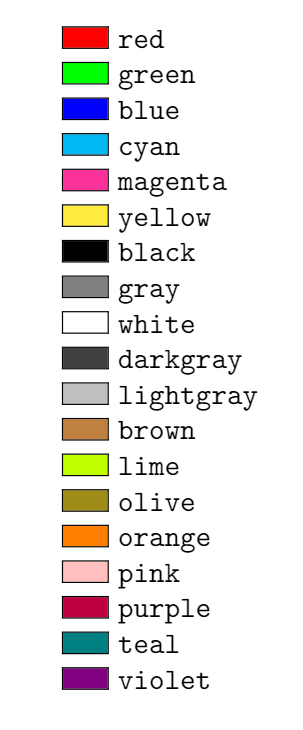
\includegraphics[scale=0.5]{OLxcolorList.png}
    \centering
\end{figure}

Andere Farben können so definiert werden:

\lstinputlisting[firstline=2]{settings/colors.tex}





% --------- KAPITEL ------------------

\sectionwithsubtitle{Wunderschöner \LaTeX-Zauber}{Formatierungsbeispiele}


\end{document}